\documentclass[tikz,border=10pt]{standalone}
\usepackage{tikz}
\usetikzlibrary {angles,quotes,arrows.meta, intersections, calc}
\usepackage{tkz-euclide} %for right angle marker
\usetikzlibrary{decorations.markings}
\tikzset{%
  ->-/.style={decoration={markings, mark=at position 0.95 with {\arrow{>}}},
              postaction={decorate}},
  ->>-/.style={decoration={markings, mark=at position 0.95 with {\arrow{>>}}},
               postaction={decorate}},
}


\begin{document}
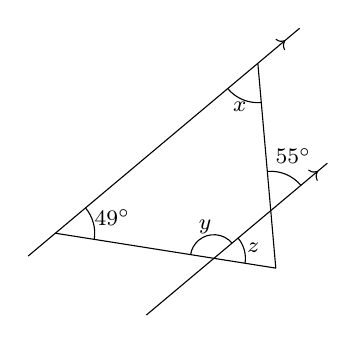
\begin{tikzpicture}[scale = 1.5]

% Draw first line at 40 degrees from horizontal
\draw[->-, name path = leg1] (0,0) -- ++(40:3cm) coordinate[pos=0.1] (C) coordinate (D);

% Draw second line parallel to the first, at a distance
\draw[->-, name path = leg2] ([shift={(1,-0.5)}]0,0) -- ++(40:2cm) coordinate (E);
%draw traversal line
\draw[name path=leg3] (C) -- ($(C)!0.7!-49:(D)$) coordinate (K);

%obtain intersection
\draw[name intersections={of=leg2 and leg3,by={M}}];
\path[name path=leg3] (K) -- ($(K)!1!-76:(C)$);
\draw[name intersections={of=leg1 and leg3,by={N}}];

\draw[name path = leg4] (K) -- (N);
\draw[name intersections={of=leg4 and leg2,by={J}}];
% % Draw the angle between lines
    \pic [draw, "\footnotesize $z$ ", angle eccentricity=1.3, angle radius=0.4cm] {angle = K--M--E};
    \pic [draw, "\footnotesize $y$ ", angle eccentricity=1.4, angle radius=0.3cm] {angle = E--M--C};
    \pic [draw, "\footnotesize $55^\circ$ ", angle eccentricity=1.5, angle radius=0.5cm,] {angle = E--J--N};
    \pic [draw, "\footnotesize $49^\circ$ ", angle eccentricity=1.5, angle radius=0.5cm,] {angle = K--C--N};
    \pic [draw, "\footnotesize $x$ ", angle eccentricity=1.2, angle radius=0.5cm,] {angle = C--N--K};

\end{tikzpicture}
\end{document}


